\documentclass[10pt, conference]{IEEEtran}
\usepackage[english]{babel}
\usepackage[usenames]{color}
\usepackage{colortbl}
\usepackage{comment}
\usepackage{graphicx}
\usepackage{epsfig}
\usepackage{array, colortbl}
\usepackage{listings}
\usepackage{epstopdf}
\usepackage{multirow}
\usepackage{rotating}
%\usepackage{subfigure}
\usepackage{subfig}
\usepackage{float}
\usepackage[obeyspaces,hyphens,spaces]{url}
\usepackage{balance}
\usepackage{fancybox}
\usepackage{scalefnt}
\usepackage[normalem]{ulem}
%\pagestyle{plain}
\pagenumbering{arabic}
\pagestyle{empty}
\clubpenalty = 10000
\widowpenalty = 10000
\displaywidowpenalty = 10000
\usepackage{cleveref}

\makeatletter
\renewcommand{\paragraph}[1]{\noindent\textsf{#1}.}

\newcommand{\rqone}{%
    \textit{%
        RQ1: What are the characteristics of in-range updates that break a client’s build?
    }
}
\newcommand{\rqtwo}{%
    \textit{%
        RQ2: How do clients respond to in-range breaking updates?
    }
}
\newcommand{\rqthree}{%
    \textit{%
        RQ3: Do broken builds in clients prompt a response from the breakage-inducing provider?
    }
}

\title{
    Keeping The Build Up-To-Par\\
    \huge An empirical study on in-range breaking updates in the npm ecosystem
}
\author{Benjamin J. Rombaut$^{1}$
    \\
    \emph{
        $^{1}$ School of Computing, Queen's University, Canada
    }
}

\begin{document}
\maketitle

\begin{abstract}
Software dependency relationships allow a client package to reuse certain versions of a provider package. These provider packages often release versions containing bug fixes, new functionalities, and security enhancements, so it is important for the clients to keep their dependencies up to date. Client's can specify a range of versions from providers they would like to accept, usually including small upgrades and fixes, which will automatically be installed whenever the client's project is built. However, these in-range updates can sometimes break a client's build, which is problematic as users of the client package will also automatically receive the in-range update and not be able to build the client's project. To understand the characteristics of these in-range breaking updates and how they are resolved, we examine in-range breaking build issue reports opened by the Greenkeeper bot and actions that are taken by clients to get their build passing again. We find that the majority of issues are created for patch updates, and that packages with higher total and more frequent releases tend to cause more breakages. Often, the client simply updating their dependency specifications is enough for them to resolve their build, and we found no indication that releases that break a relatively high proportion of client's builds prompts a response in the provider packages.
\par
Source-code Link: \url{https://github.com/brombaut/LOG6307_Project} 
\end{abstract}
\begin{IEEEkeywords}
    Dependency Management, Software Ecosystems, Breaking changes
\end{IEEEkeywords}

\section{Introduction}
\label{sec:introduction}
%describe why it is important to analyze the proposed research project
Today's software systems are large and complex. They are rarely built from scratch, and it is commonplace for developers to leverage others' code that has been built in the past to facilitate code reuse. Prior research shows that code reuse is related to the improvement of developers productivity, software quality, and time-to-market of software products \cite{FSE2017_Abdalkareem_WhyUseTrivialPackages} \cite{ESE2020_Abdalkareem_ImpactOfUsingTrivialPackages}. However, this often comes at an increased cost of having to manage these dependencies \cite{ACM2017_Mirhosseini_AutomatedPullRequests}.
\par
Greenkeeper\footnote{https://greenkeeper.io/} is a popular automated dependency management tool that GitHub\footnote{https://github.com/} and npm\footnote{https://www.npmjs.com/} users can integrate into their projects. Each time one of their dependencies releases a new version, Greenkeeper opens a new branch with that update. If the repositories continuous integration pipeline fails with the new dependency version and the dependency release is an in-range update, Greenkeeper will open up an issue report in the client’s repository with information stating which dependency update caused the problem.
\par
These in-range updates that break client's builds should not be overlooked. Semantic versioning\footnote{https://semver.org/} works so that clients can specify a range of versions they would like to be able to use from a provider. This is done so that they can automatically receive simple bug fixes and patch updates as the provider releases them. If Greenkeeper is opening an issue report for an in-range update that is breaking a client's build, it means that if a user of the client's package were to download and install the package after the dependency has released their in-range update, or even  simply try to update the dependencies on the client's project, it would fail to build. Therefore, it is expected that there would be a certain level of urgency from practitioners when they receive these issue reports.
\par
In our study, we examine these in-range breaking build issues to determine characteristics that cause these build failures, as well as how client’s respond to these issues and how they resolve their build. Specifically, we investigate the following research questions: 
\begin{itemize}
    \item \rqone
    \item \rqtwo
    \item \rqthree
\end{itemize}
\par
%describe your contributions and finding if applied
%describe the structure of the paper (follow any reference paper mentioned in class)
The remainder of this paper is structured as follows. 
We start by describing the background information in Section~\ref{sec:background}. 
% Section ~\ref{sec:approach} provides an overview of the study design. 
Section~\ref{sec:data} discusses the data set we used for the study. 
Section~\ref{sec:results} presents the results of our research questions. 
Section~\ref{sec:threats} presents the threats to validity of our study.
The related work is presented in Section~\ref{sec:relatedwork}. 
Finally, Section~\ref{sec:conclusion} draws conclusions and discusses future work.

\section{Background}
\label{sec:background}
%describe the methodology background or domain background. Imagine a non-expert will read your paper and what he/she needs to know in order to follow your work. 
%Describe the background of your work (if applied). For instance, if you expect readers understand forking behaviors of GitHub and you are afraid that some of them do not have the background knolwedge, you can describe the background here. If you believe that majority of your audience understand the context. You don't need a background section.
In this section, we provide a more in-depth description of dependency-relationships, semantic versioning, and Greenkeeper.
% Dependency relationships
~\subsection{Dependency Relationships}
\label{sec:background.dependencies}
Software dependency relationships allow a client package to reuse a certain version of a provider package stored in online package distributions. There are over 1.6 million packages available on npm alone\footnote{https://libraries.io/npm}. These provider packages are constantly evolving, with newly added features and patches that fix bugs in older versions. Additionally, the availability of such a huge amount of reusable packages facilitates software development and evolution. However, dependency relationships can also cause problems, such as software becoming out of date with respect to more recent package releases, or, if the packages are kept up-do-date, there is a risk that the new version will break existing functionality, so developers may resort to version pinning their dependencies or other less-than-ideal solutions \cite{2019CogoDowngrades} \cite{2017_Kula_DoDevsUpdateTheirDependencys}.
% Semantic Versioning and Dependency Constraints
~\subsection{Semantic Versioning and Dependency Constraints}
\label{sec:background.semver}
With many software packages being created and updated every day, it is important to standardize the way of versioning and keeping track of package releases and dependencies. Semantic Versioning, referred as \textit{semver}, has become a popular policy for communicating the kinds of changes made to a software package. It allows dependent software packages to be informed about possible “breaking changes”. A semver-compatible version is a version number composed of a major, minor and patch number. The version numbers allow to order package releases. For example, 1.2.3 occurs before 1.2.10 (higher patch version), which occurs before 1.3.0 (higher minor version), which occurs before 2.1.0 (higher major version). Backward incompatible updates should increment the major version, updates respecting the API but adding new functionalities should increment the minor version, while simple bug fixes should increment the patch version. Unfortunately, the semantic versioning policy is not always respected by package maintainers.
\par
\textbf{npm} recommends software packages to follow a specific flavor of semantic versioning\footnote{https://docs.npmjs.com/misc/semver}. Package releases specify their version number in the metadata stored in a json file\footnote{https://docs.npmjs.com/files/package.json}, and use dependency constraints to specify the version ranges of other packages they depend upon. These constraints are built from a set of operators that specify versions that satisfy the range. Table \ref{tab:semver} summarizes the types of dependency constraints for npm, their interpretation and an example of each constraint type.
\begin{table*}[h]
    \begin{center}
    \begin{tabular}{ c|c|c|c } 
         \textbf{Constraint} & \textbf{Interpretation} & \textbf{Example} & \textbf{Satisfied Versions} \\
        \hline
        fixed & exact version required & =2.3.1 & 2.3.1 \\ 
        \hline
        minimal & only use releases above the declared version & $>$=2.3.0 & $\geq$2.3.0 \\ 
        \hline
        maximal & only use releases below the declared version & $<$2.3.1 & $<$2.3.1 \\ 
        \hline
        latest & use latest available release & latest & $\geq$0.0.0 \\ 
        \hline
        hyphen ranges & only use releases between two versions & 1.2.3-2.3.4 & $\geq$1.2.3 $\land$ $\leq$2.3.4 \\ 
        \hline
        x ranges & only update where "x" or "*" is & 1.2.x & $\geq$1.2.0 $\land$ $<$1.3.0 \\ 
        \hline
        tilde ($\sim$) & only update patches & $\sim$2.3.0 & $\geq$2.3.0 $\land$ $<$2.4.0 \\ 
        \hline
        caret ($\string^$) & only update patches and minor releases & $\string^$2.3.0 & $\geq$2.3.0 $\land$ $<$3.0.0 \\ 
    \end{tabular}
    \end{center}
    \caption{
        \label{tab:semver}Types of dependency constraints for npm package dependencies
    }
\end{table*}
% Greenkeeper
~\subsection{Greenkeeper and In-Range Issues}
\label{sec:background.greenkeeper}
As previously mentioned, Greenkeeper is a tool that practitioners can integrate with their project and has been shown to be an effective tool for dependency management. Projects that use Greenkeeper upgraded 1.6x as often as projects that did not use any tools \cite{ACM2017_Mirhosseini_AutomatedPullRequests}. It sits between npm and GitHub,  watching the modules their repository depends on. Each time one of the dependencies is updated, Greenkeeper opens a new branch with that update. The repository’s CI tests run, and Greenkeeper watches the results to see whether they pass or not. Based on the test results and the  client’s dependency version definitions, Greenkeeper will open an issue report in the client’s repository with information stating which dependency update caused the problem. Figure \ref{fig:gk_issue_report} shows an example of an issue report opened by Greenkeeper.
\begin{figure}[h]
    \centering
    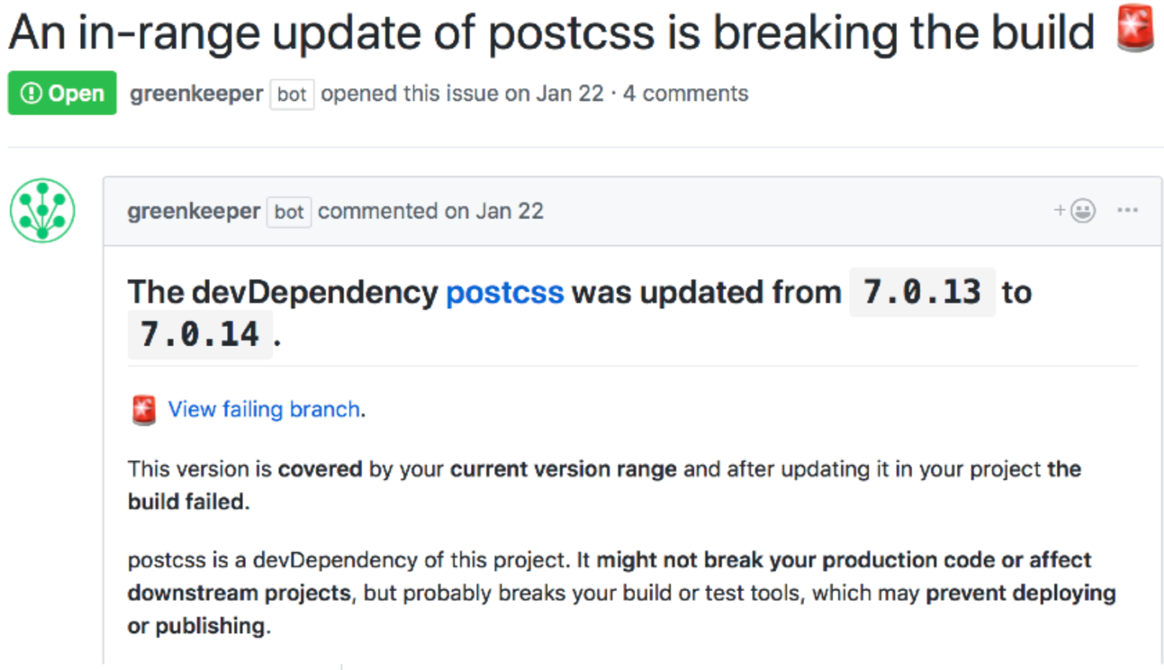
\includegraphics[width=8cm]{images/gk_issue.png}
    \caption{A Greenkeeper in-range issue report}
    \label{fig:gk_issue_report}
\end{figure}
\par
An in-range update means that a client will accept the update without having to change their version specification. For example, If a client specifies an accepted version range of $\string^$1.0.0 for a dependency, and that dependency releases version 1.0.1, that update is in-range. Users of the client's package would receive this update when they run \textit{npm install}. If an update is out of range of a client's version specification, they will not receive the update. So if an an out-of-range update breaks a client, their user's will not be effected. 





% \section{Approach}
% \label{sec:approach}
% In this section, we discuss how we collected the data set used in this study.



\section{Data Set}
\label{sec:data}
%provide an overview of the data collection process (figures are preferred) 
In this section, we discuss how we collected the data set used in this study.
\begin{figure*}[h]
    \centering
    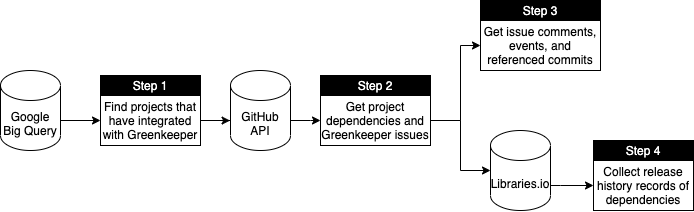
\includegraphics[width=12cm]{images/data_collection.png}
    \caption{Data collection overview}
    \label{fig:data_collection}
\end{figure*}
\par
~\subsection{Greenkeeper Issue Reports}\label{sec.data.issue_reports}
We use Google Big Query\footnote{https://cloud.google.com/bigquery} to find 12,134 GitHub projects that have integrated with Greenkeeper. From this list of repositories, we use the GitHub API\footnote{https://docs.github.com/en/free-pro-team@latest/rest} to retrieve the repository information, including the projects development and run-time dependency version specifications, as well as all of the issue reports for the project authored by the Greenkeeper bot. This leaves us with 123,197 in-range breaking build issue reports. For each of these issue reports, we collect any comments that have been made on the issue report, as well as any events that occurred on the issue report. Issue events\footnote{https://docs.github.com/en/free-pro-team@latest/rest/reference/issues\#events} can be any actions that concerns the event, such as closing an issue or referencing the event on a pull request. In total, we collect 365,625 comments and 209,750 issue events. If there were any commits that referenced the issue report, we collect information on those commits, for a total of 17,623 commits.
~\subsection{Provider Package Releases}\label{sec.data.provider_releases}
After each of the projects development and run-time dependencies had been extracted, we collected each of the dependencies release history from \textit{libraries.io}\footnote{https://libraries.io/}. In total, we collect information on 556,742 releases across 7,361 unique dependencies.
\par
An overview of the data collection process is shown in Fig.~\ref{fig:data_collection} and the data set is summarized in Table \ref{tab:all_data}.
\begin{table}[h]
    \begin{center}
    \begin{tabular}{ c|c } 
        \textbf{Entity} & \textbf{Records} \\
        \hline
        Projects & 12,134 \\
        \hline
        In-range breaking build issue reports & 123,197 \\
        \hline
        Issue comments & 365,625 \\ 
        \hline
        Issue events & 209,750 \\ 
        \hline
        Referenced commits& 17,623 \\ 
        \hline
        Release Versions & 556,742 \\ 
        \hline
    \end{tabular}
    \end{center}
    \caption{
        \label{tab:all_data} Summary of data
    }
\end{table}



\section{Results}
\label{sec:results}
% Present the results for the original paper's RQs on the new data set.


%describe the setup of your experiment, e.g., the parameters of your model, how you split train-test, what are your baselines, evalution metrics, etc. 

In this section, we present the results of our empirical study with respect to our three research questions. For each research question, we present our motivation, approach, and results.
% \subsection{Experiment Setup}
\subsection{\rqone}
\label{sec:results:rq1}
\subsubsection{Motivation}
In this research question, we look to see whether there are any common characteristics of packages that release in-range breaking updates, and what types of updates end up breaking a client's build. In-range breaking updates are problematic for clients and finding common features of these updates is the first step in attempting to eliminate them.

\subsubsection{Approach}
We first wanted to see how the in-range breaking updates were distributed across different update types. Recall that semantic versioning splits updates into three primary categories: \textit{patch}, \textit{minor} and \textit{major} updates. On the breaking build issue reports, we extract the version the dependency was being updated from and the version the dependency was being updated to in order to determine whether the release was a major, minor, or patch update. We also want to compare how the number of in-range breaking updates by type compare to how often these update types are being released, as well as how often these update types are actually accepted by client version specifications.
\par
To determine what proportion each update type has of all releases, we examine all of the versions each of the dependency to determine how many patch, minor, and major updates the package has released. We determined what types of updates clients accept from providers by extracting each client's development and run-time dependency version specifications, and determining the type of updates they accept based on the rules outlined in Table \ref{tab:semver}.
\par
Another factor we investigate was whether the release frequency of provider packages tends to have any affect on how often they release in-range updates that break their clients. We tally the number of in-range updates each provider has that broke their client's, and compare the distributions across the total number of releases that package has, as well as the frequency at which that package releases new versions.

\subsubsection{Results}
We were able to extract the version ranges of the breaking dependency being updates for 63.77\% of the issue reports. This is because Greenkeeper will bundle upgrades for the packages that have to be upgraded together, and if one of the updates in the bundle breaks the client's build, the issue report is opened for all of the updates in the bundle. We are not able to determine the specific breaking dependency in the bundle, and we therefore omit these issue reports from our analysis.
\par
We found that 65.15\%, 34.69\%, and 0.16\% of in-range breaking updates are patch, minor, and major updates, respectively. These results would suggest that package developers are not following the semantic versioning scheme, which states that only major updates should be used to signify a breaking change in the package. However, patch and minor updates occur much more frequently than major updates. We found that 64.37\%, 28.25\%, and 7.37\% of package releases were patch, minor and major updates, respectively. This explains to some degree why the number of in-range breaking updates that are patch and minor updates is larger than major updates, since patch and minor updates occur more frequently then major updates.
\par
Additionally, we found that major updates are far less likely to be accepted as in-range updates by clients. Recall that, in order for an update to be considered in-range, the client must specify the range of updates they are willing to accept. We found that 12.53\% of dependencies are pinned by clients, which means the provider will never be able to release an in-range update. Of the remaining dependencies, 3.74\%, 82.31\%, and 1.08\% are accepting patch, minor, and major updates, respectively, which would further reduce the number of major updates that are considered to be in-range for clients. These results are summarized in Figure \ref{fig:bar_stacked_breaks_releases_accepted_update_types}
\begin{figure}[h]
    \centering
    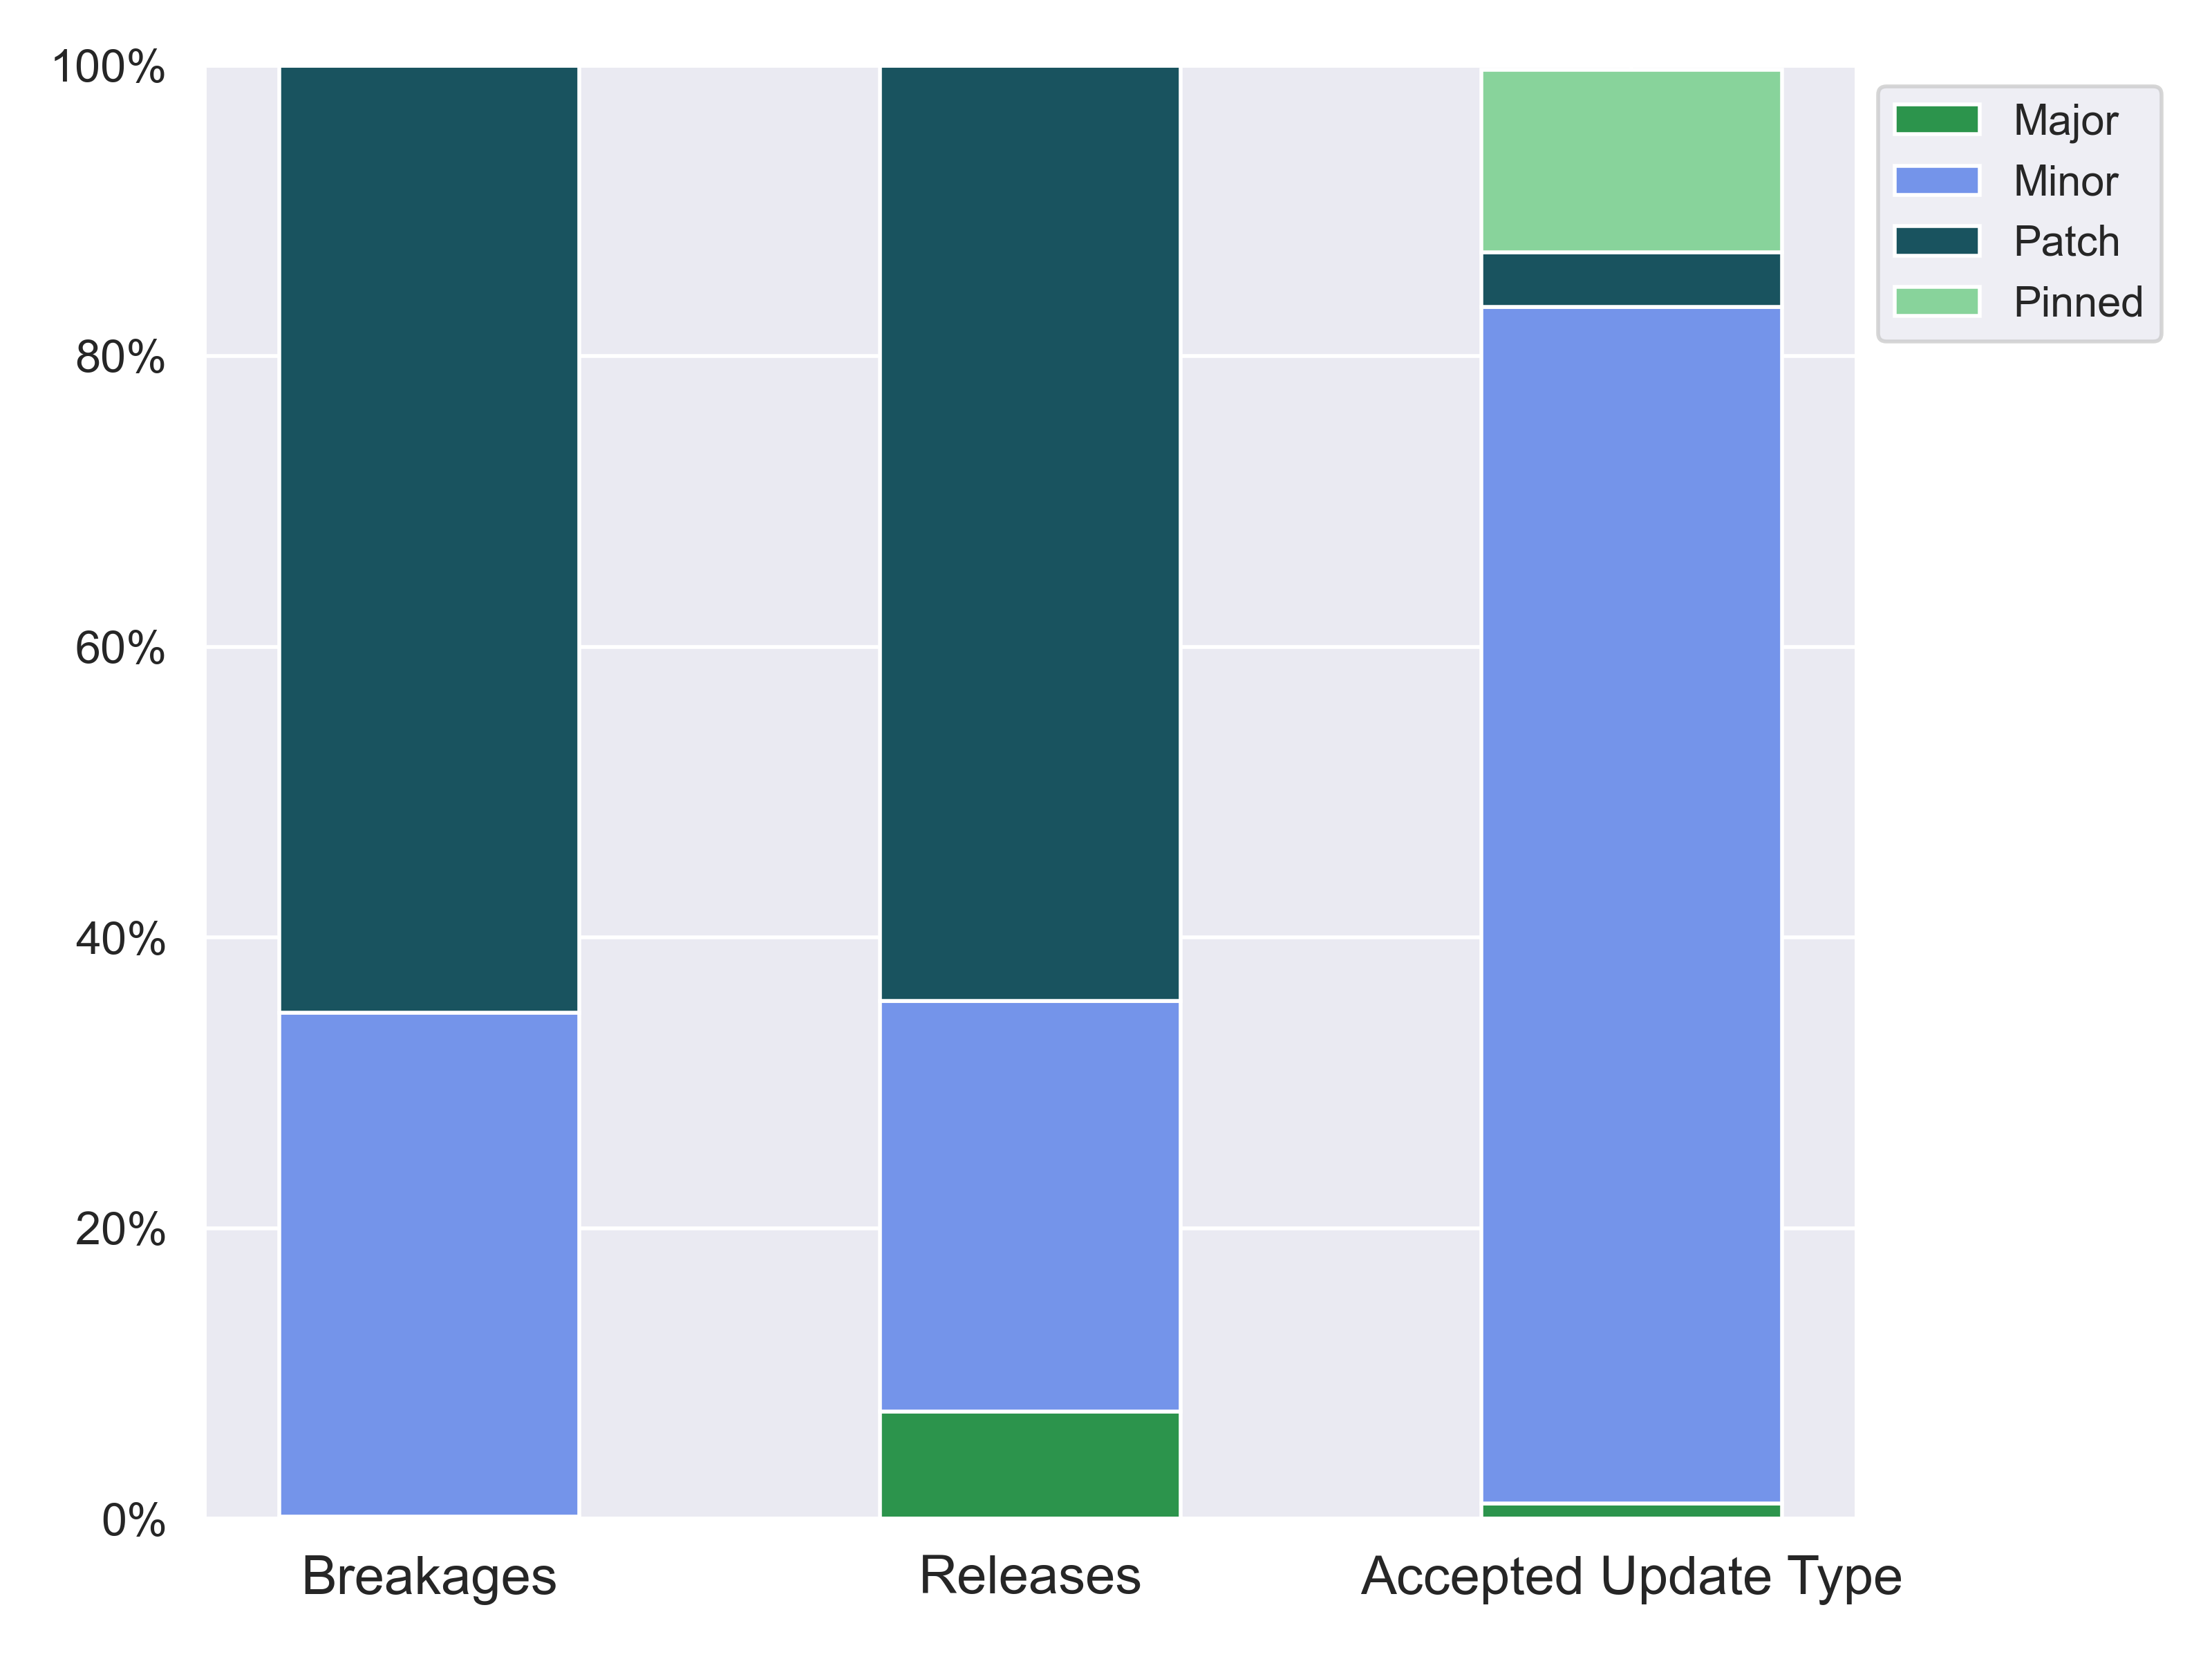
\includegraphics[width=\linewidth]{images/rq1_stacked.png}
    \caption{Distribution of update types for in-range breakages, package releases, and accepted update types}
    \label{fig:bar_stacked_breaks_releases_accepted_update_types}
\end{figure}
\par
In terms of how the release practices of packages affect how often they release in-range breaking updates, we found that the number of broken builds increases by 0.07 for every additional release a package makes. Intuitively, this result is expected. The more releases a package has, the more opportunities there are that a release will break a client's build. We also look at the distribution of build breakages caused by a provider against the frequency at which they release new versions. We found that the number of in-range breakages decrease by $3.7e-10$ as the release frequency increases, which is not strong evidence that a higher release frequency is less likely to cause in-range breaking updates, or vice versa. These results are visualized in Figure \ref{fig:dist_breaks_to_package_release_total_and_freq}.
\begin{figure*}[h]
    \centering
    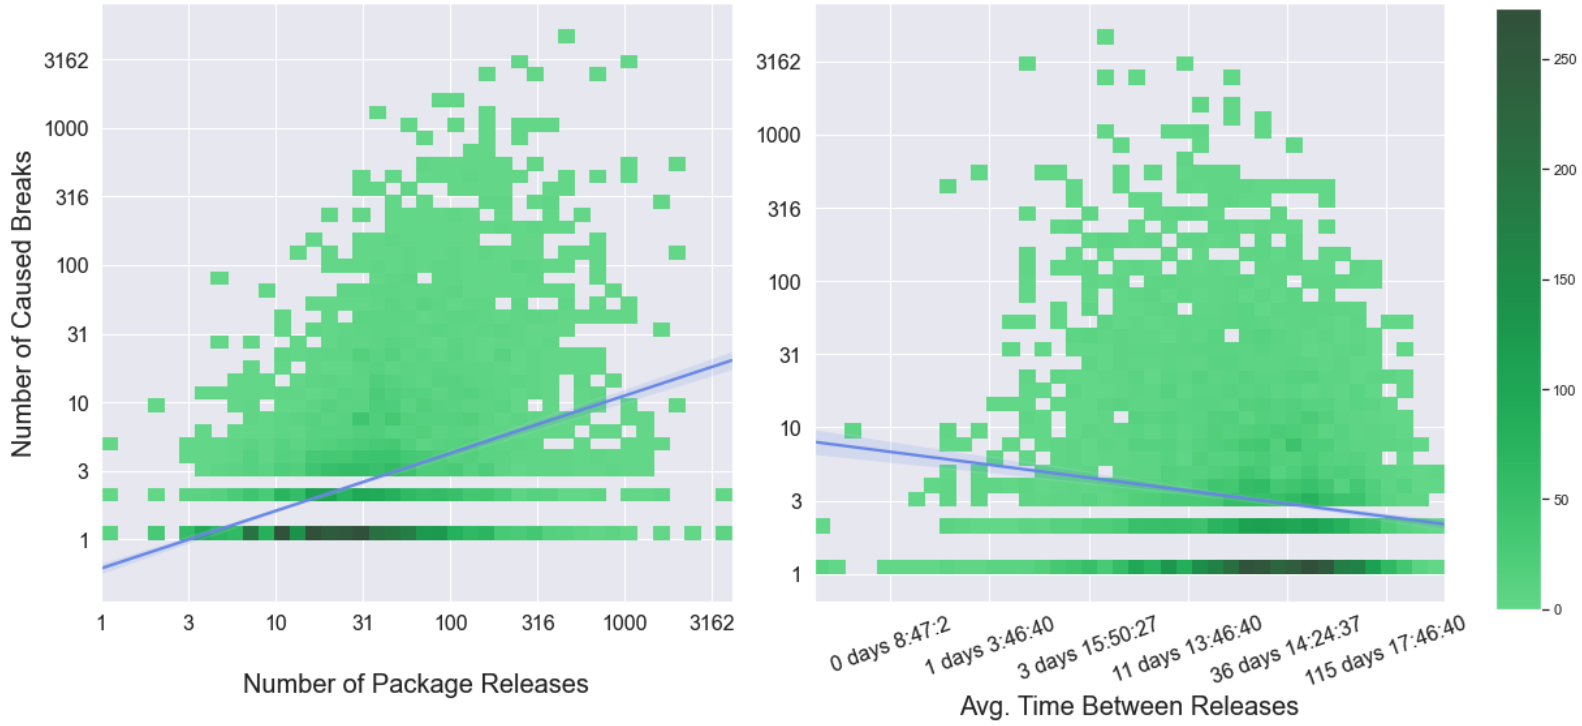
\includegraphics[width=15cm]{images/breakages_to_package_releases_and_frequency_manual.png}
    \caption{Distribution of number of cause breakages and total package releases (left) and release frequency (right)}
    \label{fig:dist_breaks_to_package_release_total_and_freq}
\end{figure*}
\newline
\par
\fbox{%
    \parbox{8cm}{%
        While the majority of clients will accept minor updates, most breakages are caused by patch updates. Packages with higher total and more frequent releases tend to cause more breakages.
    }%
}
\subsection{\rqtwo}
\label{sec:results:rq2}
\subsubsection{Motivation}
As previously mentioned, in-range breaking updates should be treated with a sense of urgency by client developers, as any attempt by users to install their package after the in-range dependency update will fail. In this research question, we look at how client developers respond to these in-range updates, and what actions they have to take in order to resolve their build.

\subsubsection{Approach}
To answer this research question, we examine a number of attributes related to the in-range breaking build issue reports opened in the client projects. We look at the content of the issue reports themselves, the comments on the issue reports, as well as the types of changes that are made by developers in order to fix their builds, Additionally, we look at the effectiveness of Greenkeeper's automatic attempts at pinning the breaking dependency as a first attempt to resolve the client's build.

\subsubsection{Results}
We found that 79.82\% of in-range breaking update issue reports were eventually closed, with a median time to close the issue of 4 days and 11 hours. We examine the comments on in-range breaking build issue reports in order to gain insight into how clients are responding to these issues. We found that 85.93\% of issues have at least 1 comment. This is expected, as Greenkeeper will attempt to pin the breaking dependency immediately after opening the majority of issue reports, and will automatically comment the build result of pinning the dependency on the issue report. 47.95\% of issues have at least 2 comments. We hypothesised that approximately half of all comments on the issue reports were from users. However, further analysis revealed that only 2.93\% of comments were from non-bot users on GitHub, and that 96.89\% of all comments are from the Greenkeeper bot itself, with the remaining comments being from other bots.
\par
Specifically examining the user comments, we found that the median response time was 2 days and 12 hours. We classified these comments using regular expressions to match specific phrases and patterns. We found that users are specifically referencing a fix for the issue 34.5\% of the time, while the simply mention the issue has been fixed 17.4\% of the time. 18.3\% of comments indicate the build failure is a false alarm, referencing a flaky test, CI hiccup, or that they simply re-ran the build pipeline and it passed without incident. The proportion of user comment types, as well as the average response times for each type are summarized in Figure \ref{fig:issue_comments}
\begin{figure*}[h]
    \centering
    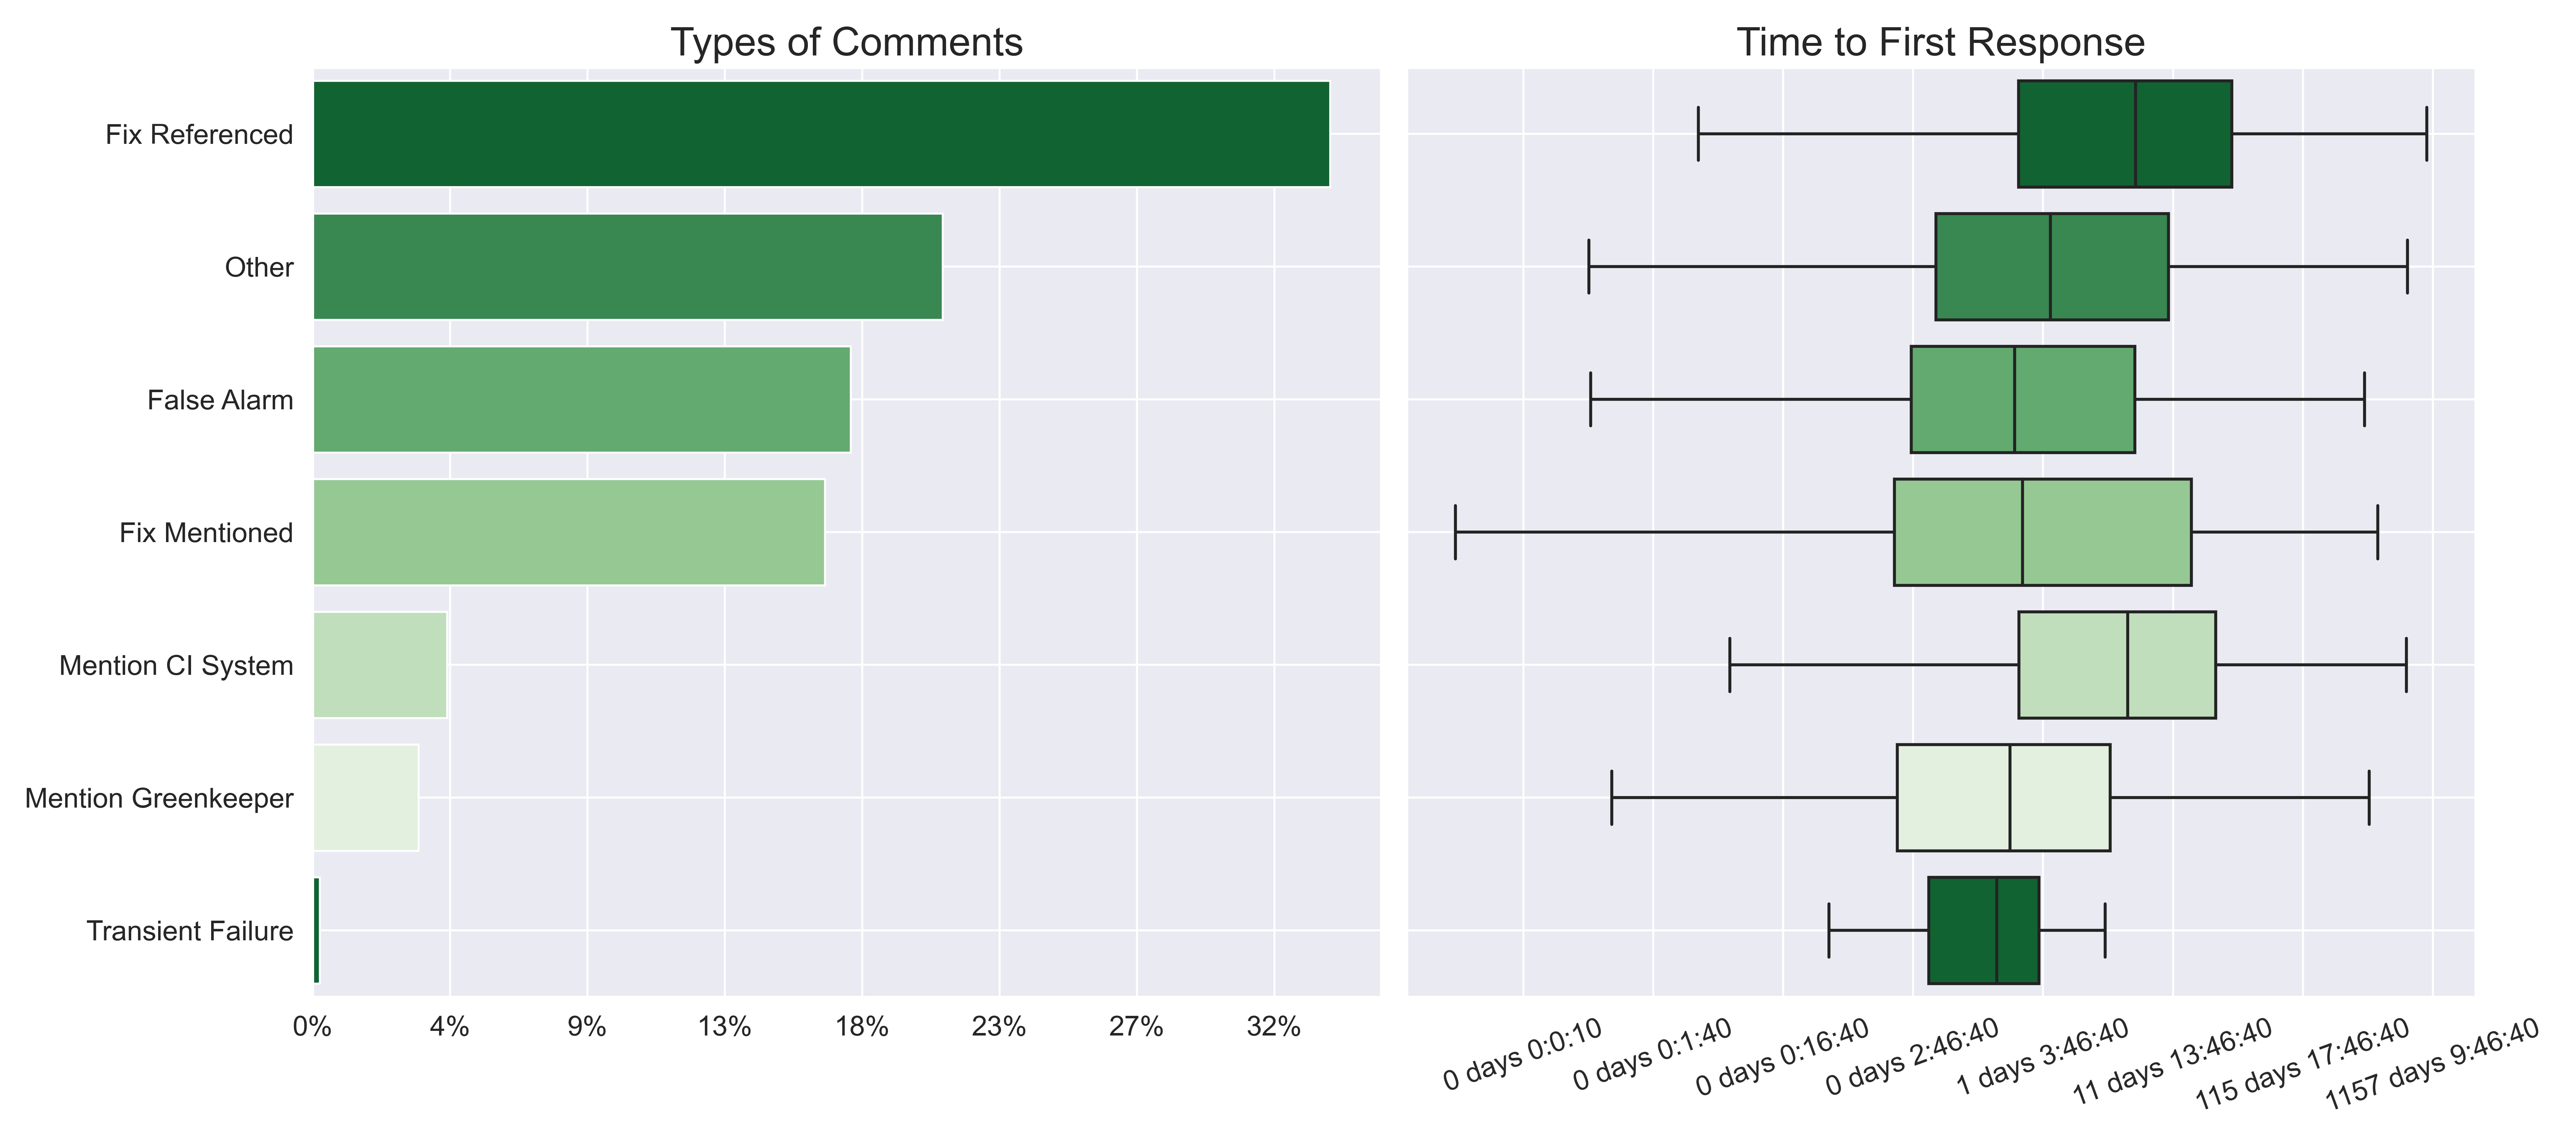
\includegraphics[width=16cm]{images/types_of_comments_and_time_until_comment_type.png}
    \caption{Most common types of comments left by users on in-range breaking build issue reports (left) and how long users take to make each response (right) }
    \label{fig:issue_comments}
\end{figure*}
\par
We saw that practitioners were referencing fixes on these issue reports, so we investigated what these fixes entail. We found that 69.7\% of referenced commits include changes the \textit{package.json} file, 28.5\% include changes to the \textit{package-lock.json} file, and 25.6\% include changes to the \textit{yarn.lock} file. These are all files that are used to specify a projects dependencies. The two lock files are automatically generated and so have a relatively high commit churn, with the \textit{package-lock.json} file having a median commit churn of 101 additions and 130 deletions, and the \textit{yarn.lock} having a median commit churn of 44 additions and 59.5 deletions. However, the \textit{package.json} file, which is manually maintained, has a median commit churn of 1 addition and 1 deletion per commit when fixing an in-range breaking build issue. This suggests that, in order to fix their build, users are simply updating their accepted dependency version range, such as pinning the dependency that is failing the build. Figure \ref{fig:changed_files} summarized the most common files changed in referenced commits on in-range breaking build issues, as well as their commit churn. Additionally, these results shows that it is uncommon for clients to modify their source code that uses these dependencies in order to fix their builds.
\begin{figure*}[h]
    \centering
    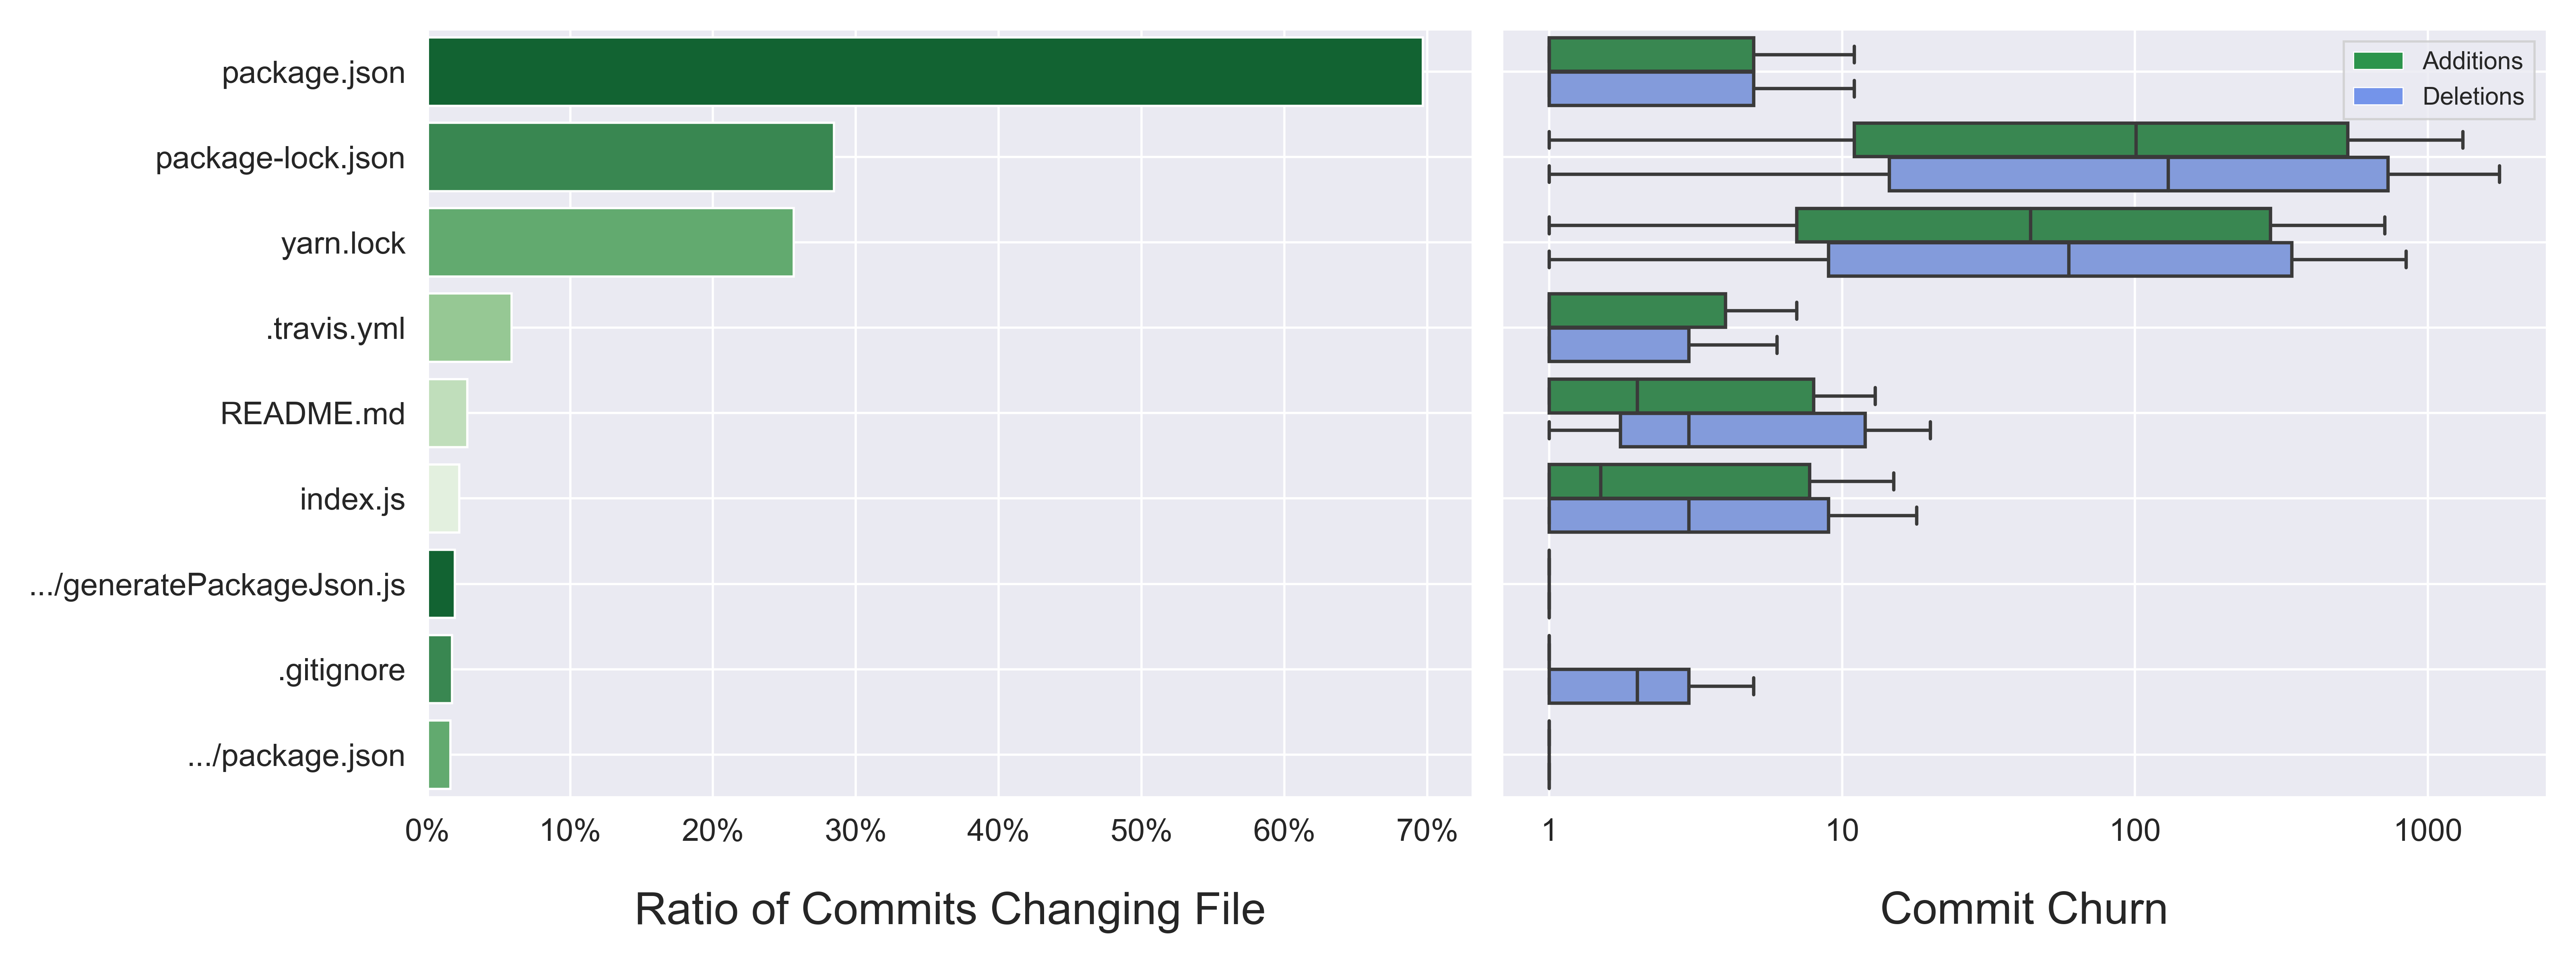
\includegraphics[width=\linewidth]{images/changed_files_ratio_and_commit_churn.png}
    \caption{Most common files changed in commits referenced by in-range breaking build issue reports (left) and the commit churn of each file (right)}
    \label{fig:changed_files}
\end{figure*}
\par
When the Greenkeeper bot opens a breaking build issue report, it will automatically attempt to pin the dependency to the previous version and re-run the build to determine if the issue can be resolved. Pinning a dependency is a legitimate option when developers don’t have the time or resources to fix a problem introduced by a dependency update. Greenkeeper will bundle upgrades for the packages that have to be upgraded together, and it won’t attempt to pin all of the packages in the bundle, which is why 28.1\% of issues don’t have a pin attempt. However, of the issue reports that did have a pin attempt, only 33.1\% resulted in the client's build passing again. This indicates that the majority of these in-range breaking build update issue reports are not actually caused by the dependency being updated. In order to better understand the reasons as to why so many pin attempts fail, we manually analyze a sample of the issue reports that have a failed pin attempt. We found that clients improperly configuring their projects build pipeline was the primary reason for the dependency updates failing, including missing configuration files, invalid credentials, or inconsistent environment versions. We also saw that the builds can fail due to flaky tests, request timeouts, and even  attempting to run the build before the branch had been created in the project repository.
\par
Additionally, we found that Greenkeeper does not take into account the type of error that occurs in the pipeline when testing new dependency updates, and will consider any error that occurs in the pipeline as a build failure. This means that, for example, if a developer that does not conform to the project's linter configuration, then all subsequent builds will fail, and Greenkeeper will open in-range breaking update issue reports for any dependencies that release a new in-range version. If the dependency continues to release new versions, the issue report will become flooded with comments from Greenkeeper confirming that the build is still failing, introducing a lot of noise into projects and distracting from valid issue reports, which practitioners say is one of the main reasons for not using automated dependency management tools \cite{ACM2017_Mirhosseini_AutomatedPullRequests}.
\newline
\par
\fbox{%
    \parbox{8cm}{%
        The majority of client responses mention a fix or confirm the issue is invalid. Most fixes involve small changes to dependency specification files. While pinning the dependency is a legitimate option, it is not as successful as expected due to builds failing for reasons not related to the dependency being updated.
    }%
}
\subsection{\rqthree}
\label{sec:results:rq3}
\subsubsection{Motivation}
In the previous research question, we looked at how clients respond to in-range breaking updates. However, while it is the client's build that is failing, the root cause of the issue could originate from the provider. In this research question, we look to see whether in-range breaking updates prompt a response from the provider packages.
\subsubsection{Approach}
Initially, we examined all of the comments made by users on the in-range breaking build issue reports looking for potential references to issue report made in the dependency package that were related to the client's breaking build issue report. We were not successful in finding any, so we took a different approach. We hypothesis that, if a release from a package provider causes an in-range breaking builds in a high proportion of client, the next release the provider package makes would happen quicker than usual. To test this, we compare the average release frequency of packages against the time it takes a package to release the next update immediately following an update that causes an in-range breaking build in at least 20\% of clients that depend on it.
\par
First, we determine the number of clients that are using each of the provider packages we have release information on in our data set. We then determine how many issue reports were opened for each release made by each provider package. Using this information, we determine the ratio of in-range breaking update issue reports that each release made by every provider package caused. This allows us to categorize each release either as a breaking release or a non-breaking release. We then compare the release frequency of the non-breaking releases to the time to the release immediately following each breaking release.

\subsubsection{Results}
We first used all release records in our analysis including releases that did not cause any in-range update breaking issues in any clients. We found that the median release time after non-breaking releases was 1 day and 22 hours (IQR = 3 hours - 10 days 12 hours), while the median release time immediately following a breaking release was 8 days and 6 hours (IQR = 1 day and 3 hours - 39 days and 6 hours). From these results, it appears that the release that immediately follow an update that breaks a proportion of clients tends to take longer to be made available. However, we choose to perform further analysis on only breaking releases.
\par
We examine only the set of releases that caused at least one in-range breaking build issue report to be opened in a client. While all these releases caused at least one breaking build, we still classify a breaking release as a release that caused at least 20\% of the package's client's builds to break. The median release time immediately following a breaking release was still 8 days and 6 hours (IQR = 1 day and 3 hours - 39 days and 6 hours), as that data set was unaffected, but the median release time after non-breaking releases was 8 days and 6 hours (IQR = 1 day 3 hours - 39 days 6 hours). These results can be seen in Figure \ref{fig:time_until_next_breaking_release}.
\begin{figure*}[h]
    \centering
    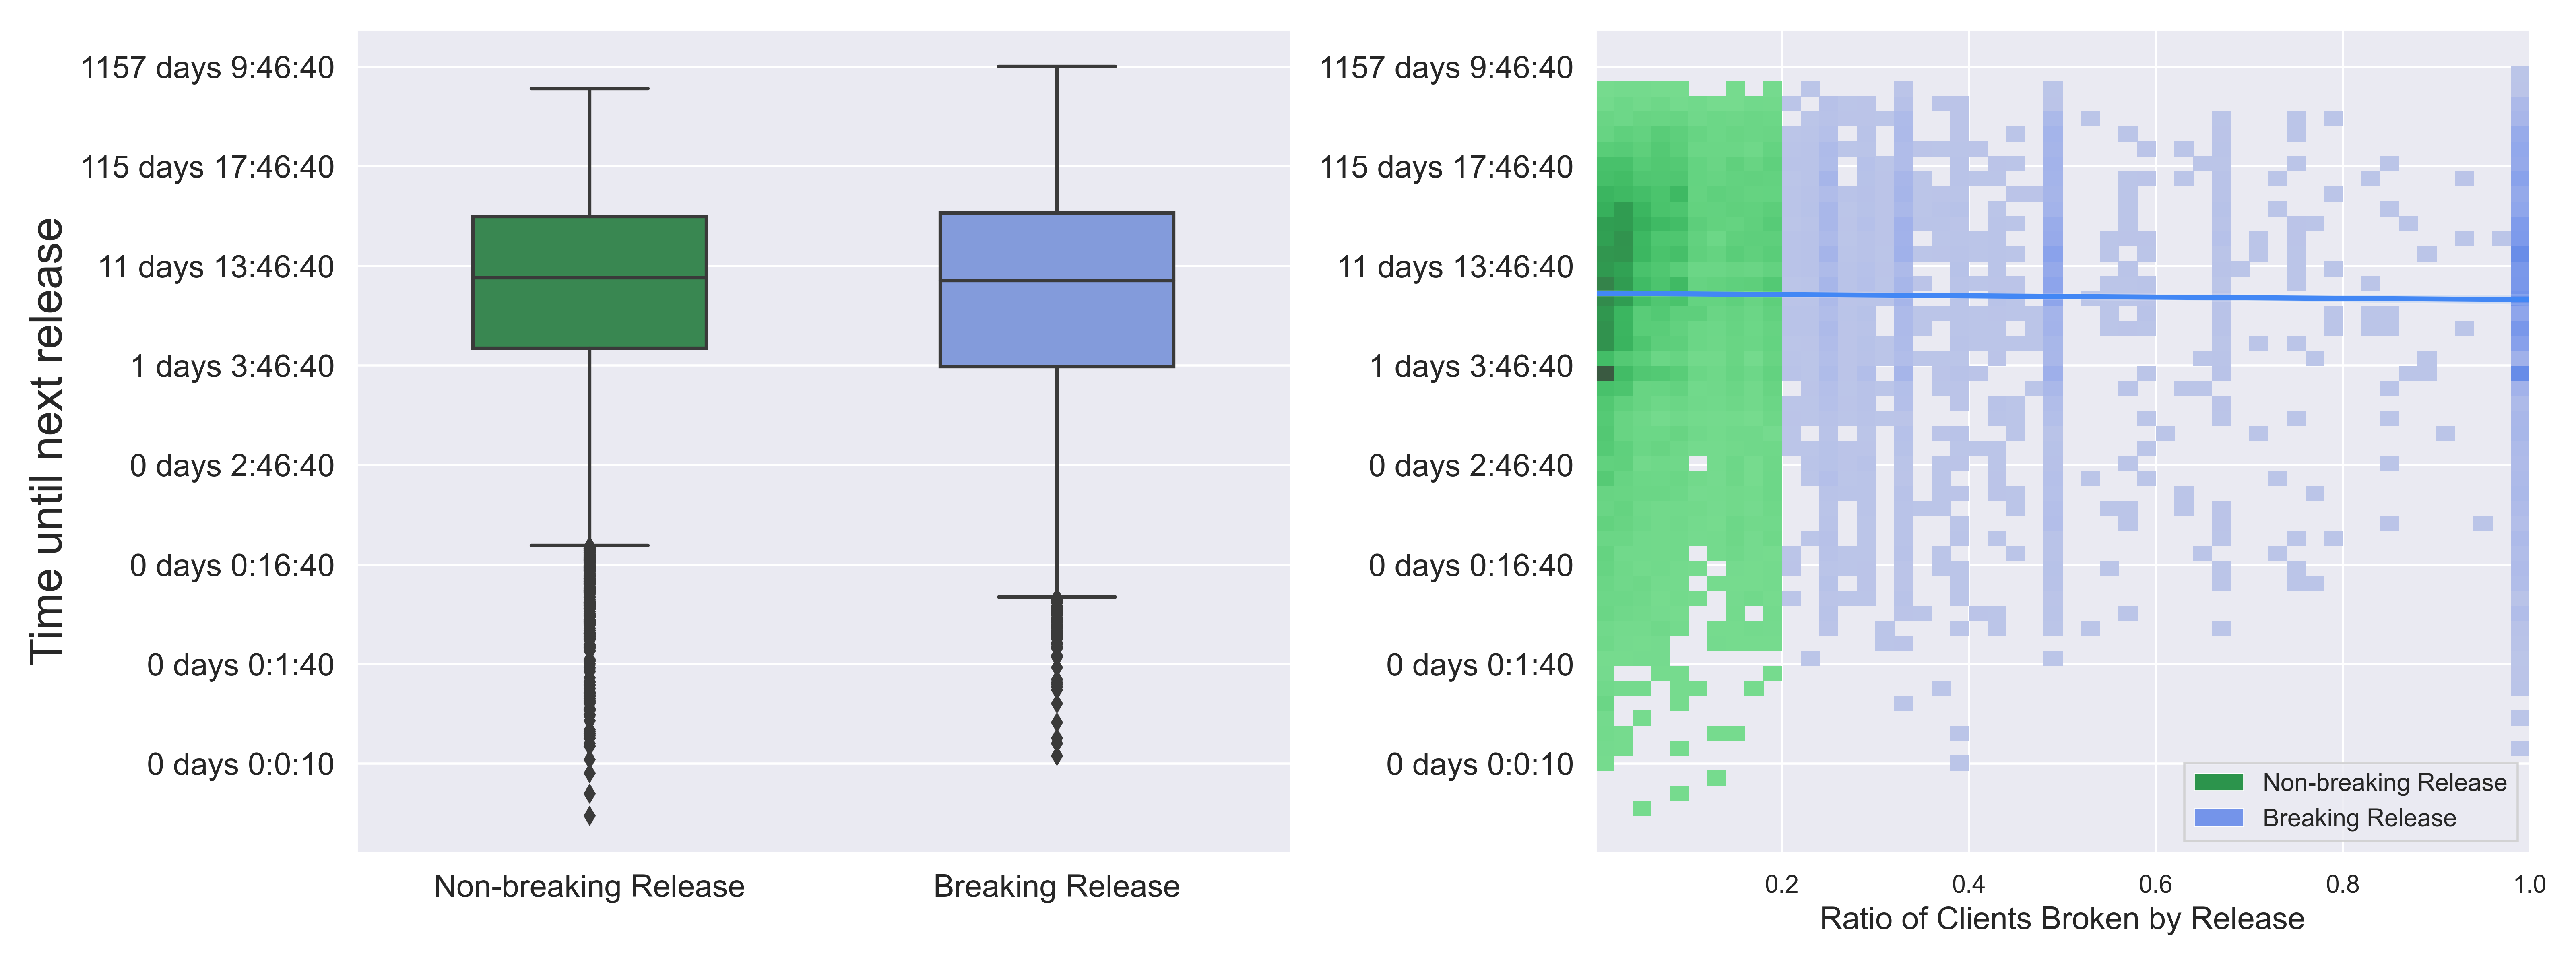
\includegraphics[width=\linewidth]{images/time_until_next_release_after_break_plots.png}
    \caption{Time until next release for non-breaking and breaking releases}
    \label{fig:time_until_next_breaking_release}
\end{figure*}
\newline
\par
\fbox{%
    \parbox{8cm}{%
        We did not find any indication that client's are filing issue reports with provider packages that release in-range breaking updates. There is no statistical difference that indicates that breaking releases are immediately followed up by a quicker release than normal.
    }%
}


% \section{Comparison of Results}
% \label{sec:comparison-results}

% Second most important section of a replication study, in which the results are compared to the original study's results to understand whether the original approach generalizes to the new data set, and, if not, why? Go deeper than just "values are different'', i.e., why would that be the case? What other case study should one do to validate your explanation?

\section{Threats to Validity}
\label{sec:threats}
%describe the internal and external threats to validity (ref. https://www.verywellmind.com/internal-and-external-validity-4584479)
In this section, we disuses threats to validity that might influence our study.
\subsection{Threats to Internal Validity}
Internal validity concerns factors that could have influenced our analysis and findings. First, we did not perform any filtering of either the client projects or the provider packages we examined, such as removing inactive or "toy" projects. This may have affected our results pertaining how clients respond to the in-range breaking update issue reports, as well as the results involved with the release frequency of providers.
\par
We only collect a single snapshot of each client's dependencies, and therefore we do not have the dependency history of each client project in our data set. In other words, we do not know at what date a client project integrates with each of it's dependencies, or whether they remove any dependencies over their lifetime. We therefore assume that a client uses each of the dependencies for it's lifetime for our analysis in Section \ref{sec:results:rq3}. This may have biased our results when classifying each provider release as either a breaking or non=breaking release based on the ratio of client each released caused an issue report to be created.

\subsection{Threats to External Validity}
Threats to external validity concern the generalization of our technique and findings. First, we only analyse projects that have integrated with the Greenkeeper bot. While Greenkeeper is a popular tool used by many projects \cite{ACM2017_Mirhosseini_AutomatedPullRequests}, they might not be representative of the general population, and while we analyzed a large sample of open-source repositories, these results may not extend to proprietary systems, which may operate under different constraints. Further, Greenkeeper was acquired by Snyk\footnote{https://snyk.io/} in June 2020, and is no longer monitoring projects for in-range breaking updates. Additionally, one of the prerequisites for clients integrating with Greenkeepepr is that the project must have a \textit{package.json} file specifying it's dependencies. This means that Greenkeeper is only able to monitor dependencies in the \textit{npm} ecosystem for in-range breaking updates. Therefore, our analysis only examines npm packages, which can include many new and evolving packages. The dynamic nature of JavaScript can result in harder to detect breaking changes, which may be less of concern in other languages and ecosystems.
\par
Finally, while performing our manual analysis to determine why so many attempts at pinning the dependency being updated did not resolve the client's build, we did not analyze enough samples to be statistically significant. We only analyzed a total of 50 sample, and while they all failed for similar reasons, this is not a statistically significant sample size, and might not lead to generalizable results.

\section{Related Work}
\label{sec:relatedwork}
%briefly categorize the existing related work 
%describe at least three most relevant related work in details (what they did and findings, how it is similar or different from your work).
In this section, we present the work most related to our study. 
% We divide the prior work into two main areas; work related to the study of API breakage changes and API testing.

\par
Mirhosseini et al. ~\cite{ACM2017_Mirhosseini_AutomatedPullRequests} conducted a study on why developers neglect to update software dependencies, and how effective Greenkeeper and other automated tools are at helping developers keep their dependencies up to date. They found these tools to be useful, with projects that use pull request notifications upgraded on average 1.6x as often as projects that did not use any tools. They also found that, although pull request notifications are useful, developers are often overwhelmed by notifications: only a third of pull requests were actually merged. Through a survey of developers, they found  that one of the primary reasons why practitioners don’t update their dependencies is due to the fear of breaking changes. This demonstrates a need for better tools that give developers higher confidence that updating their dependencies will not break their code.

\par
Xavier et al. \cite{SANER2017_Xavier_HistoricalImpactAnalyisOfAPIBreakingChanges} performed a large-scale study on the historical and impact analysis of API breaking changes in the Java ecosystem. They assess the frequency of breaking changes, the behavior of these changes over time, the impact on clients, and the characteristics of libraries with high frequency of breaking changes. Alongside their results, they provide a set of lessons to better support library and client developers in their maintenance tasks. One of their more interesting results is that, despite their findings that 28\% of all API changes break backwards compatibility, only 2.54\% of clients are potentially impacted.

\par
Brito et al.\cite{ESE2020_Brito_YouBrokeMyCode} conducted a follow up survey to their 2018 paper that introduced \textit{APIDIFF}, a tool to identify API breaking and non-breaking changes between two versions of a Java library \cite{SANER2018_Brito_APIDiff}. After identifying possible breaking changes, they asked the developers to explain the reasons behind their decision to change the APIs, and find that breaking changes are mostly motivated by the need to implement new features, by the desire to make the APIs simpler and with fewer elements, and to improve maintainability. To complement this first study, they conduct an analysis of 110 Stack Overflow posts related to breaking changes. they find that breaking changes have an important impact on clients, since 45\% of the questions are from clients asking how to overcome specific breaking changes.


\section{Conclusion}
\label{sec:conclusion}
It has become commonplace for developers to reuse code from multiple provider packages, and clients will often specify a range of versions they would like to use from provider packages so that they can automatically receive simple bug fixes and patch updates as the provider releases them. However, these in-range updates can sometimes break a client's build, and since the dependency update is accepted in the client's version specifications, the client package will also not build for any of it's users. In this study, we examined breaking build issue reports created by the Greenkeeper bot for in-range updates to determine characteristics that cause these build failures, as well as how client’s respond to these issues and how they resolve  their build. We found that the majority of issues are created for patch updates, and that packages with higher total and more frequent releases tend to cause more breakages. Often, the client simply updating their dependency specifications is enough for them to resolve their build, and we found no indication that releases that break a relatively high proportion of client's builds prompts a response in the provider packages.



\balance
\bibliographystyle{IEEEtran}
\bibliography{assignment.bib}
\end{document}
